\documentclass{beamer}
\usefonttheme[onlymath]{serif}

\setbeamersize{text margin left=1.5em}
\setbeamersize{text margin right=1.5em}




\setbeamertemplate{frametitle}{%
  \vskip1ex
  \usebeamerfont{frametitle}%
  \insertframetitle\par %frame 에서 지정한 title 사용
  %\insertsubsectionhead\par        % subsection의 header를 사용
  \vskip1ex
  \hrule                             % 밑줄(선택)
}

\setbeamertemplate{blocks}[rounded][shadow=true] % 블록 테두리 둥글게

\setbeamertemplate{itemize item}{\usebeamerfont{itemize item}\textbullet}
\setbeamertemplate{itemize subitem}{\usebeamerfont{itemize subitem}\textbullet}
\setbeamertemplate{itemize subsubitem}{\usebeamerfont{itemize subsubitem}\textbullet}



%\setbeamerfont{itemize/enumerate subbody}{parent=itemize/enumerate body} % 
%\setbeamerfont{itemize/enumerate subbody}{size=\usebeamerfont{itemize/enumerate body}\size}

\makeatletter
% Taken from beamer.cls' default geometry settings
% http://mirrors.ctan.org/macros/latex/contrib/beamer/base/beamer.cls
\geometry{%
  papersize={\fpeval{\beamer@paperwidth*1.35}pt,\fpeval{\beamer@paperheight*1.35}pt},
  hmargin=\fpeval{0.5 * 1.35}cm,% 1cm
  vmargin=0cm,%
  head=\fpeval{0.5*1.35}cm,% 0.5cm
  headsep=0pt,%
  foot=\fpeval{0.5*1.35}cm% 0.5cm
}
\makeatother %from search keyword beamer size, get this search result -> https://tex.stackexchange.com/questions/586756/beamer-use-glyphs-from-smaller-font-size-but-enlarge


% Reference bibtex
% style = numeric, apa, authoryear-comp
\usepackage[backend=biber, style=authoryear-comp, natbib=true]{biblatex}
\addbibresource{../../references.bib}



% 테마 선택 (선택 사항)
% \usetheme{Madrid} % 기본 테마, 다른 테마 사용 가능
% \font{serif}
\usepackage{amsfonts}
\usepackage{amssymb}
\usepackage[T1]{fontenc} % To use combination of textbf, textit
\usepackage[dvipsnames]{xcolor}   % can use more variant colors
%\usepackage{lmodern} %다른 폰트 사용: 문서의 서문에 추가하면 Computer Modern 폰트의 확장 버전인 Latin Modern 폰트를 사용할 수 있습니다. 이 폰트는 더 다양한 크기와 스타일을 지원하여 문제를 해결해 줄 수 있습니다.

% \setcounter{MaxMatrixCols}{20}

% (필요한 패키지들)
% \usepackage{amsthm}
\setbeamertemplate{theorems}[numbered]  % 정리, 정의 등에 번호를 달아줌

% \theoremstyle{plain} % insert bellow all blocks you want in italic
% \newtheorem{theorem}{Theorem}[section] % to number according to section
% 
% \theoremstyle{definition} % insert bellow all blocks you want in normal text
% \newtheorem{definition}{Definition}[section] % to number according to section
% \newtheorem*{idea}{Proof idea} % no numbered block

\newtheorem{proposition}[theorem]{Proposition}

\usepackage{tcolorbox}

% 필요할 경우 패키지 추가
\usepackage{graphicx} % 이미지 삽입을 위한 패키지
\usepackage{amsmath}   % 수식 사용
\usepackage{hyperref}  % 하이퍼링크 추가
\hypersetup{colorlinks} % search keyword: beamer hyperref color -> https://tex.stackexchange.com/questions/13423/how-to-change-the-color-of-href-links-for-real
\usepackage{cleveref}
\usepackage{multicol}  % 여러 열 나누기
\usepackage{ulem} % 취소선 및줄 나누기
\usepackage{mathtools} % dcases
%\usepackage{xparse} % NewDocumentCommand
\usepackage[boxed, lined]{algorithm2e} % to use algorithm block



% \NewDocumentCommand{\DefThreeOp}{m}{%
%   % \csname #1\endcsname 라는 이름으로, 3개 인자를 받는 새 매크로를 정의
%   \expandafter\NewDocumentCommand\csname #1\endcsname{mmm}{%
%     \operatorname{#1}\!\bigl(##1,\,##2,\,##3\bigr)%
%   }%
% }

\newcommand{\mrm}[1]{\mathrm{#1}}
\newcommand{\mbb}[1]{\mathbb{#1}}
\newcommand{\mb}[1]{\mathbf{#1}}
\newcommand{\mc}[1]{\mathcal{#1}}
\newcommand{\tb}[1]{\textbf{#1}}
\newcommand{\ti}[1]{\textit{#1}}
\newcommand{\Pois}[1]{\operatorname{Pois}(#1)}

\newcommand{\myber}[1]{\operatorname{Bern}\!\left(#1\right)}
\newcommand{\Bin}[2]{\operatorname{Bin}\!\left(#1,#2\right)}
\newcommand{\NBin}[2]{\operatorname{NBin}\!\left(#1,#2\right)}
\newcommand{\mytoinf}[1]{#1 \rightarrow \infty}
\newcommand{\myexp}[1]{\exp{\left(#1\right)}}
\newcommand{\Unif}[2]{\operatorname{Unif}\!\left(#1, #2\right)}
\newcommand{\mygeom}[1]{\operatorname{Geom}\!\left(#1\right)}
\newcommand{\Expo}[1]{\operatorname{Expo}\!\left(#1\right)}
\newcommand{\abs}[1]{\left\lvert #1 \right\rvert}
\newcommand{\floor}[1]{\left\lfloor #1 \right \rfloor}
\newcommand{\expec}[1]{\operatorname{E}\left[ #1 \right]}
\newcommand{\Var}[1]{\operatorname{Var}\left[#1\right]}
\newcommand{\myskew}[1]{\operatorname{Skew}\!\left[#1\right]}
\newcommand{\mykurt}[1]{\operatorname{Kurt}\!\left[#1\right]}
\newcommand{\mywei}[2]{\operatorname{Wei}\!\left(#1, #2\right)}
\newcommand{\Span}{\operatorname{Span}}
\newcommand{\Cov}[2]{\operatorname{Cov}\!\left(#1, #2\right)}
\newcommand{\intinfty}{\int_{-\infty}^\infty}
\newcommand{\Corr}[2]{\operatorname{Corr}\!\left(#1, #2\right)}
\newcommand{\Mult}[3]{\operatorname{Mult}_{#1}\!\left(#2, #3\right)}
\newcommand{\Beta}[2]{\operatorname{Beta}\!\left(#1, #2\right)}
\newcommand{\HGeom}[3]{\operatorname{HGeom}\!\left(#1, #2, #3\right)}
\newcommand{\NHGeom}[3]{\operatorname{NHGeom}\!\left(#1,#2, #3\right)}
\newcommand{\GammaDist}[2]{\operatorname{Gamma}\!\left(#1, #2\right)}
%\DefThreeOp{PHGeom}

\newcommand{\im}{\operatorname{im}}
\newcommand{\tr}{\operatorname{tr}}


% 발표 제목, 저자, 날짜 설정
\title{Domain Randomization}
\author{Gwanwoo Choi}
% \date{}

\begin{document}
% 표지 슬라이드

\begin{frame}
    \titlepage
\end{frame}

% \subsection{Domain Randomization}
% \begingroup
%     \setbeamertemplate{frametitle}{%
%     \vskip1ex
%     \usebeamerfont{frametitle}%
%     \insertframetitle\par        %  ← 원하는 대로 변경 가능
%     \vskip1ex
%     \hrule                             % 밑줄(선택)
%     }
%     \begin{frame}
%         \frametitle{Table of Contents}
%         \tableofcontents[currentsubsection]
%     \end{frame}
% \endgroup

% % 목차 

% \begin{frame}{Curriculum Learning}

% \end{frame}

\begin{frame}{Domain Randomizaiton}
    \begin{itemize}
        \item In sim-to-real problem, dynamics parameters are unknown to the agent at inference time.
        \begin{figure}
            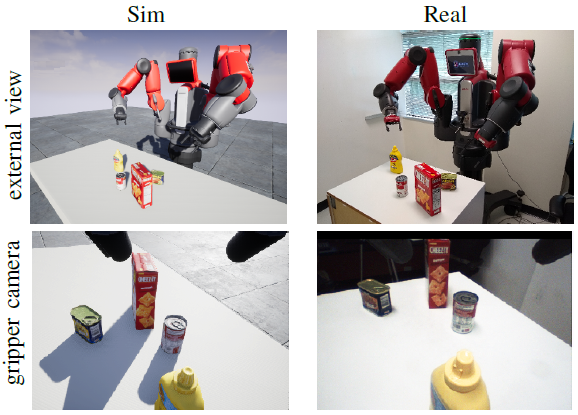
\includegraphics[width=0.45\textwidth]{sim2real.png}
        \end{figure}
        \item \tb{Domain Randomization} is one of the most popular algorithms for sim-to-real transfer and requires no interaction with the real-world environment.
        \item Unlike a traditional MDP setting, domain randomization varies the simulation environment with an environment parameter $\xi \in \Xi$.
        \begin{itemize}
            \item For example, in the Cart-Pole task, there are parameters such as \ti{pole mass}, \ti{car mass}, and \ti{slider-cart friction}.
        \end{itemize}
        \item Domain randomization varies the environment parameters, and agent training takes place in each environment.
    \end{itemize}
\end{frame}

\begin{frame}{Domain Randomization}
    \begin{block}{Domain Randomization}
        \begin{itemize}
            \item Let $\Xi$ denote the domain randomization parameter space, and $\xi \in \Xi$ denote each domain randomization parameter.
            \item In domain randomization MDP is considered of the form $\mc{M}_\xi = (\mc{S}, \mc{A}, T_\xi, R_\xi, \gamma)$.
            \item Each MDP $\mc{M}_\xi$ shares the same state space, action space, and reward function, but differs by transition dynamics and reward function.
            \item Transition probability $T_\xi : \mc{S} \times \mc{A} \to \mc{S}$ changes for different $\xi$.
            \item Also, reward function $R_\xi : \mc{S} \times \mc{A} \to \mbb{R}$ also changes with $\xi$.
            \item The agent interacts with environments sampled from a distribution over $\Xi$
            \item Typically, $\xi$ is sampled from probability distribution $P_\phi : \mc{S} \times \mc{A} \to [0,1]$ with parameter $\phi$
            \item The objective of domain randomization: Learns policy $\pi_\theta$ proficient on a real-world MDP $\mc{M}^\ast$ by \underline{training it purely in simulation} on a set of MDPs, $\mc{M}_\xi$.
        \end{itemize}
    \end{block}
\end{frame}


\begin{frame}{Domain Randomization}
    \begin{itemize}
        \item With policy $\pi_\theta$, we can get trajectory $\tau=\{(s_0, a_0, s_1, a_1, \dots)\}$ from each sampled MDP $\mc{M}_\xi$.
        \item Then we can set object function by
        \[
            J(\pi) = \mbb{E}_{\xi \sim P_\phi} \left[ \mbb{E}_{\tau \sim T_\xi^{\pi}}\left[\sum_{i=0}^\infty \gamma^t R_\xi (s_t, a_t) \right] \right]
        \]
        where $T_\xi^\pi (\tau) \coloneqq T_\xi (s_0) \prod_{t=0}^\infty T_\xi (s_{t+1} | s_t, a_t) \pi_\theta (a_t | s_t)$
        \item Since domain randomization is a special case of POMDPs, its optimal policy $\pi^\ast_{\text{DR}}$ in general will depend on history
    \end{itemize}
\end{frame}

\begin{frame}{Domain Randomization: \cite{curtisFlowbasedDomainRandomization2025a}}
    \begin{itemize}
        \item In [Flow-based Domain Randomization for Learning and sequencing Robotic Skills] \cite{curtisFlowbasedDomainRandomization2025a}, authors combine domain randomization technique with flow-based
        \begin{itemize}
            \item For more detail information about normalizing flow, see the \hyperlink{norm_flow}{Appendix: Normalizing Flows}
        \end{itemize}
        \item In traditional domain randomization setups, the distribution $\xi \sim P(\cdot)$ is predefined.
        \item However, selecting an appropriate $P(\xi)$ is crucial for the policy's performance and generalization
        \begin{itemize}
            \item Too broad a sampling distribution can be falls into local minima.
            \item In contrast, too narrow a sampling distribution leads to poor generalization and robustness.
            \item Additionally, rapid changes to the sampling distribution can lead to unstable training.
        \end{itemize}
    \end{itemize}
\end{frame}

\begin{frame}{Domain Randomization: \cite{curtisFlowbasedDomainRandomization2025a}}
    \begin{itemize}
        \item In this paper, propose method named \tb{GoFlow}, which has following objective function
        \[
            \max_{P, \pi} \{\mbb{E}_{\xi \sim P_{\phi}} [J_\xi (\pi)] + \alpha \mc{H}(P) - \beta D_{KL}(P_{\text{old}}\parallel P)\}
        \]
        where
        \[
        \begin{gathered}
            \mbb{E}_{\xi \sim P_\phi(\xi)}[J_\xi(\pi)] = \int_\Xi P_\phi(\xi) J_\xi (\pi) d\xi \\
            \mc{H}(P_\phi) = - \int_\Xi P_\phi(\xi)\log P_\phi(\xi) d\xi \\
        \end{gathered}
        \]

        \begin{itemize}        
            \item For samplied $\xi \sim P_\phi$, policy $\pi_\theta$ should obtain high rewards.
            \item At the same time, $P_\phi$ should be sample broader range of parameter $\xi$, by $\mc{H}(P_\phi)$.
            \item Concurrently, for stabilized training, $D_{KL}(P_{\text{old}}\parallel P)$ constrains $P$ to not deviate significantly from $P_{old}$.
        \end{itemize}
        \item In implementation, employ the PPO algorithm (\cite{schulmanProximalPolicyOptimization2017}), an on-policy policy gradient method that optimizes a stochastic policy while ensuring stable efficient learning
        \begin{itemize}
            \item To further stabilize training, they priviliged information about the environment parameters $\xi$ to the critic network, parametrized by $\psi$.
        \end{itemize}
        \[
            V_\psi(s_t, \xi) = \mbb{E}_{\pi_\theta} \left[\sum_{k=0}^\infty \gamma^k r_{t+k} \middle| s_t, \xi \right]
        \]

    \end{itemize}
\end{frame}

\begin{frame}{Domain Randomizaiton: \cite{curtisFlowbasedDomainRandomization2025a}}
    % \begin{figure}
    %     \includegraphics[width=0.5\textwidth]{GoFlowAlgorithm.png}
    % \end{figure}
    \[
        \max_{P, \pi} \{\mbb{E}_{\xi \sim P_{\phi}} [J_\xi (\pi)] + \alpha \mc{H}(P) - \beta D_{KL}(P_{\text{old}}\parallel P)\}
    \]
    \begin{algorithm}[H]
        \IncMargin{1em}
        \SetAlgoLined
        \SetKwInOut{Require}{Require}


        \Require{Initial policy parameters $\theta$, flow parameters $\phi$, training steps $N$, network updates $K$, entropy coefficient $\alpha$, simiarlity coefficient $\beta$, and learning rate $\eta$}

        \emph{$U$ is the Uniform distribution, $\abs{\Xi}$ is finite measure of $U$}\\
        \For{$n=1$ \KwTo $N$}{
            Sample $\{\xi^{\text{train}}_i\}^B_{i=1} \sim P_\phi(\cdot)$, $\{\xi^{\text{test}}\}^B_{i=1} \sim U(\cdot)$ \\
            Train $\pi_\theta$ with initializing $\{\xi^{\text{train}}_i\}$ \\
            Estimate $J_{\xi^{\text{test}}_i}(\pi_\theta)$ via policy rollouts \\
            Save current flow distribution as $P_{\phi_{\text{old}}}$
            \For{$k=1$ \KwTo $K$}{
                $\mc{R} \leftarrow \frac{\abs{\Xi}}{B} \sum_{i=1}^B \left[ P_\phi (\xi^{\text{test}}_i) J_{\xi^{\text{test}}_i} (\pi_\theta) \right]$ \\
                $\hat{\mc{H}} \leftarrow - \frac{\abs{\Xi}}{B} \mbb{E}_{\xi \sim U} \left[ P_\phi(\xi) \log P_\phi (\xi) \right]$ \\
                $\hat{D_{KL}} \leftarrow \mbb{E}_{\xi \sim P_{\phi_{\text{old}}}}\left[ \log P_{\phi_{\text{old}}}(\xi)- \log P_{\phi}(\xi)\right]$ \\
                $\phi \leftarrow \phi + \nu \nabla_\phi (\mc{R}+\alpha \hat{\mc{H}}-\beta\hat{D}_{KL})$
            }
        }
        \caption{GoFlow Algorithm}
    \end{algorithm}
    \begin{itemize}
        \item Importance sampling \& Monte Carlo Estimation is applied for computational efficiency.
    \end{itemize}
\end{frame}

\begin{frame}{Domain Randomization: \cite{curtisFlowbasedDomainRandomization2025a}}
    \begin{figure}
    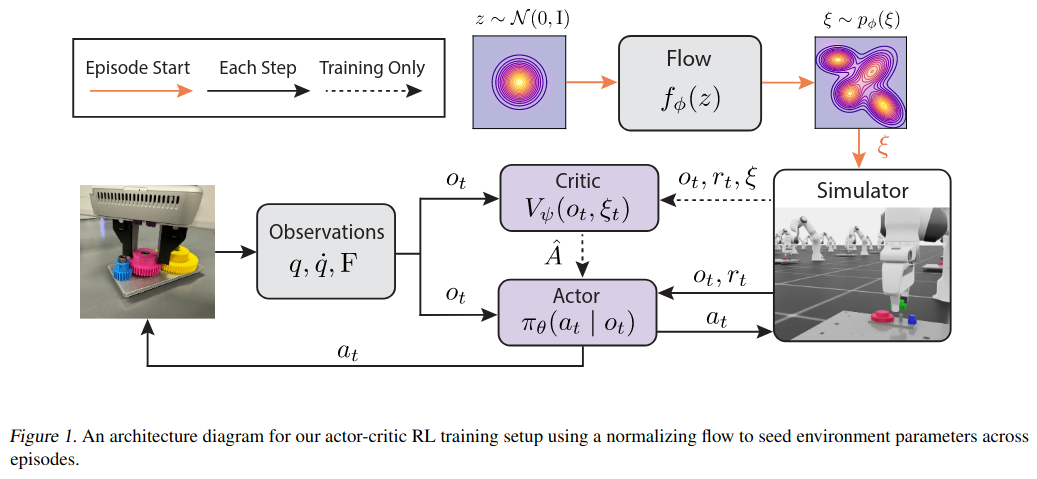
\includegraphics[width=0.8\textwidth]{GoFlowArchitecture.png}
    \end{figure}
\end{frame}


\begin{frame}{Domain Randomization: \cite{tiboniDomainRandomizationEntropy2024}}
    \begin{itemize}
        \item Domain Randomization via Maximization Entropy (\cite{tiboniDomainRandomizationEntropy2024})
        \item Given that we do not know which parameters $\xi^\ast$ corresponds to real-world MDP $\mc{M}^\ast$, we maximize the change of good performance in $\mc{M}^\ast$ by training a policy $\pi_\theta$ that generalizes well to maximum range of $\xi$.
        \item To effectively measure the degree of generalizability across $\xi$, devise a success indicator $\sigma(\tau)$ for trajectory $\tau \in \mc{T}$
        \[
            \sigma(\tau) \coloneqq \begin{cases}
                1 \text{ if } \tau \text{ is success} \\
                0 \text{ if } \tau \text{ is fail}
            \end{cases}
        \]
        \begin{itemize}
            \item  The criteria of success may be defined through, e.g., distance thresholds from a target goal location, task-specific tolerance to errors, or a lower bound on the expected return
        \end{itemize}
        \item Then success probability can be defined by
        \[
            \mc{G}(\theta, \phi) = \text{Pr}[\sigma(\tau) = 1 | \theta, \phi]
        \]
        Note that trajectory $\tau$ is random variable in above equation and sampled by values of $\theta$ and $\phi$.
    \end{itemize}
\end{frame}

\begin{frame}{Domain Randomization: \cite{tiboniDomainRandomizationEntropy2024}}
    \begin{itemize}
        \item Wider dynamics distributions $\xi \sim P_\phi(\cdot)$ will generally make it harder for the policy to keep a high success rate $\mc{G}(\theta, \phi)$.
        \item On the other hand, high variability of environments $\mc{M}_\xi$ sampled at training time will likely lead to better generalization to the real environment dynamics
        \item Following this intuition, \tb{DOmain RAndomization via Entropy MaximizaitON (DORAEMON)}, \underline{a constrained optimization problem} is formulated
        \begin{equation} \label{eq:1}
            \max_{\theta \in \Theta, \phi \in \Phi} \mc{H}(P_\phi) \text{ s.t. } \mc{G}(\theta, \phi) \geq \alpha
        \end{equation}
        where $\alpha \in [0,1]$.

        \item decouple update of $\theta$ from update of $\phi$ makes feasible to optimize, so equation \ref{eq:1} changes to
        \begin{equation} \label{eq:2}
            \max_{\phi_{i+1} \in \Phi} \mc{H}(P_{\phi_{i+1}}) \text{ s.t. } \mc{G}(\theta_i, \phi_{i+1}) \geq \alpha \ \ D_{KL}(P_{\phi_{i+1}}\parallel P_{\phi_i}) \leq \epsilon
        \end{equation}
        Where $\pi_{\theta_i}$ has been trained on dynamics $M_{\xi}$ parametrized by $\xi \sim P_{\phi}(\cdot)$.
        \item Note that, in this work, they parametrize $P_\phi$ as uncorrelated univariate Beta distributions
        \begin{itemize}
            \item With them, it is feasible to compare (distributions).
            \item In addition, dynamics parameters are often inherently bounded due to physical constraints-such as positive values for masses and friction coefficients-making beta distribution a reasonable choice
        \end{itemize}
    \end{itemize}
\end{frame}

\begin{frame}{Domain Randomization: \cite{tiboniDomainRandomizationEntropy2024}}
    \begin{algorithm}[H]
        \SetAlgoLined
        \SetKwInOut{Require}{Require}
        \SetKwInOut{Output}{Output}
        \Require{Initialize dynamics distribution $\phi_1$ policy parameters $\theta_1$, trust region size $\epsilon$, trajectories, trajectories per distribution update $K$ number of iterations $M$, success indicator function $\sigma(\tau)$}
        \Output{Generalizable policy $\pi_\theta$}

        \For{$i=1, \dots, M$}{
            Sample $K$ dynamics parameters $\{\xi_k\}_{k=1}^K, \xi_k \sim P_\phi(\cdot)$ \\
            Collect $K$ associated trajectories $\{\tau_k\}_{k=1}^K, \tau_k \sim T_\xi^{\pi_\theta}$ \\
            \tb{Policy update:} \\
            Update $\theta_{i+1}$ through any RL algorithm on collected data $\{\tau_k\}_{k=1}^K$ \\
            \tb{Dyamics distribution update:} \\
            \eIf{$\hat{\mc{G}}(\theta_i, \phi_i, \phi_i) < \alpha$}{
                Obtain $\phi_i^B$ by optimizing equation \ref{eq:4} \\
                \If{
                    $\hat{\mc{G}}(\theta_i, \phi_i, \phi_i^B) < \alpha$
                }{
                    Update $\phi_{i+1} \leftarrow \phi_i^B$\\
                    \tb{Continue}
                }
                $\phi^{\text{start}}_i \leftarrow \phi_i^B$
            }{
                $\phi^{\text{start}}_i \leftarrow \phi_i$
            }
            Obtain $P_{\phi_{i+1}}$ by optimizing equation \ref{eq:2} with $\mc{G} \approx \hat{\mc{G}}(\theta_i, \phi^{\text{start}}_i, \phi_{i+1})$ (equation \ref{eq:3})

        }
        \caption{DORAEMON algoritm}
    \end{algorithm}
\end{frame}

\begin{frame}{Domain Randomization: \cite{tiboniDomainRandomizationEntropy2024}}
    \begin{itemize}
        \item Success rate $\mc{G}(\theta, \phi)$ is equal to $\mbb{E}_{\tau} [\sigma(\tau) | \phi, \theta]$ and this is effectively distributed as a Bernoulli random variable
        \item So by Importance Sampling \& Monte Carlo Estimation, 
        \begin{equation}\label{eq:3}
        \mc{G}(\theta, \phi) \approx \hat{\mc{G}}(\theta_i, \phi_i, \phi_{i+1}) = \frac{1}{K} \sum_{k=1}^K \frac{P_{\phi_{i+1}}(\xi_k)}{P_{\phi_i}(\xi_k)} \cdot \mbb{1}_{\{\tau \in \mc{T}: \sigma(\tau)=1\}} (\tau_k)
        \end{equation}
        \item In turn, equation \ref{eq:3} allows the optimization problem in equation \ref{eq:2} to be solved using only the set of data $\{\xi_k, \tau_k\}^K_{k=1}$ naturally collected while training the policy $\pi_{\theta_i}$ for $K$ episodes.
        % \item It may occurs that $g$
        \item While convenient approximating the probability of success $\mc{G}(\theta_i, \phi_{i+1})$ through IS may lead to overestimation of the real success rate under the new distribution $\phi_{i+1}$, resulting in a violated constraint when trying to solve equation \ref{eq:2} at the next iteration
        \begin{equation} \label{eq:4}
            \phi_i^B = \arg \max_{\phi_i^\prime} \hat{\mc{G}}(\theta_i, \phi_i, \phi_i^\prime) \text{ s.t. } D_{KL}(P_{\phi^\prime_i} \parallel P_{\phi_i}) \leq \epsilon
        \end{equation}
    \end{itemize}
\end{frame}

\begin{frame}{Domain Randomization}
    \begin{center}
        \textbf{Thank you}
    \end{center}
\end{frame}

\begin{frame}{Appendix: Normalizing Flows}
    \begin{itemize}
        \item \hypertarget{norm_flow}{\tb{Normalizing Flows}} are a class of generative models that transform a simple based distribution into a complex target distribution using a sequence of invertible, differentiable functions.
        \item For example, let $z \sim p_Z(z)$ be a latent variable from a base distribution (e.g. a standard normal distribution).
        \item A normalizing flow defines an \ti{invertible transformation} $f_\phi: \mbb{R}^d \to \mbb{R}^d$ parametrized by neural network parameters $\phi$, such that $x = f_\phi(z)$, aiming for $x$ to follow the target distribution.
        \item The density of $x$ is computed using the change of variables formula, where $\frac{\partial f_\phi(z)}{\partial z}$ is the jacobian of $f_\phi$ at $z$.
        \[
            P_X(x) = P_Z(f^{-1}_\phi(x)) \abs{\det \left(\frac{\partial f^{-1}_\phi(x)}{\partial x}\right)}, \quad \log P_X(x) = \log P_Z(z) - \log \abs{\det \left(\frac{\partial f_\phi(z)}{\partial z}\right)}
        \]
        \item By composing multiple such transformations $f_\phi = f_{\phi_k} \circ \cdots \circ f_{\phi_1}$, each parametrized by neural network parameters $\phi_k$, normalizing flows can model highly complex distributions.
    \end{itemize}
\end{frame}

\begin{frame}[allowframebreaks]{References}
    \printbibliography
\end{frame}

\end{document}